\section{Edge Following}
\begin{frame}
	\frametitle{Edge Following}
		\textbf{Objective:} Algorithm to make the kilobots which are on the outer edge to move along the edge of a group of kilobots by measuring distances without being physically blocked and reach the reference bot.
\end{frame}

\begin{frame}
\frametitle{Flowchart}
\begin{figure}[H]
	\centering
	\fbox{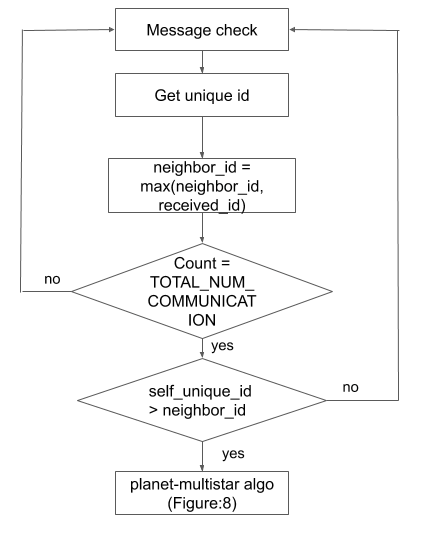
\includegraphics[scale=0.35]{images/flowchart-edge-following.png}}
	\caption{Flowchart for Edge following}
	\label{fig:Flowchart for Edge following}
\end{figure}
\end{frame}

\begin{frame}
\frametitle{Demonstration}
\begin{figure}[H]
	\centering
	    \fbox{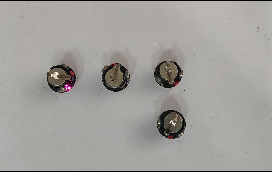
\includegraphics[width=2.5in]{images/edge-following.png}}
	    \caption{\href{https://drive.google.com/file/d/1g10OzQKxJeDGPPiBOiKoj_39G7-d5FFN/view}{Edge Following with \textit{TOTAL\_NUM\_COMMUNICATION=5} and \textit{TOTAL\_NUM\_COMMUNICATION\_ORBIT=3}}}
	    \label{fig:Edge Following}
\end{figure}
\end{frame}


